{
\usebackgroundtemplate{
	\centering
	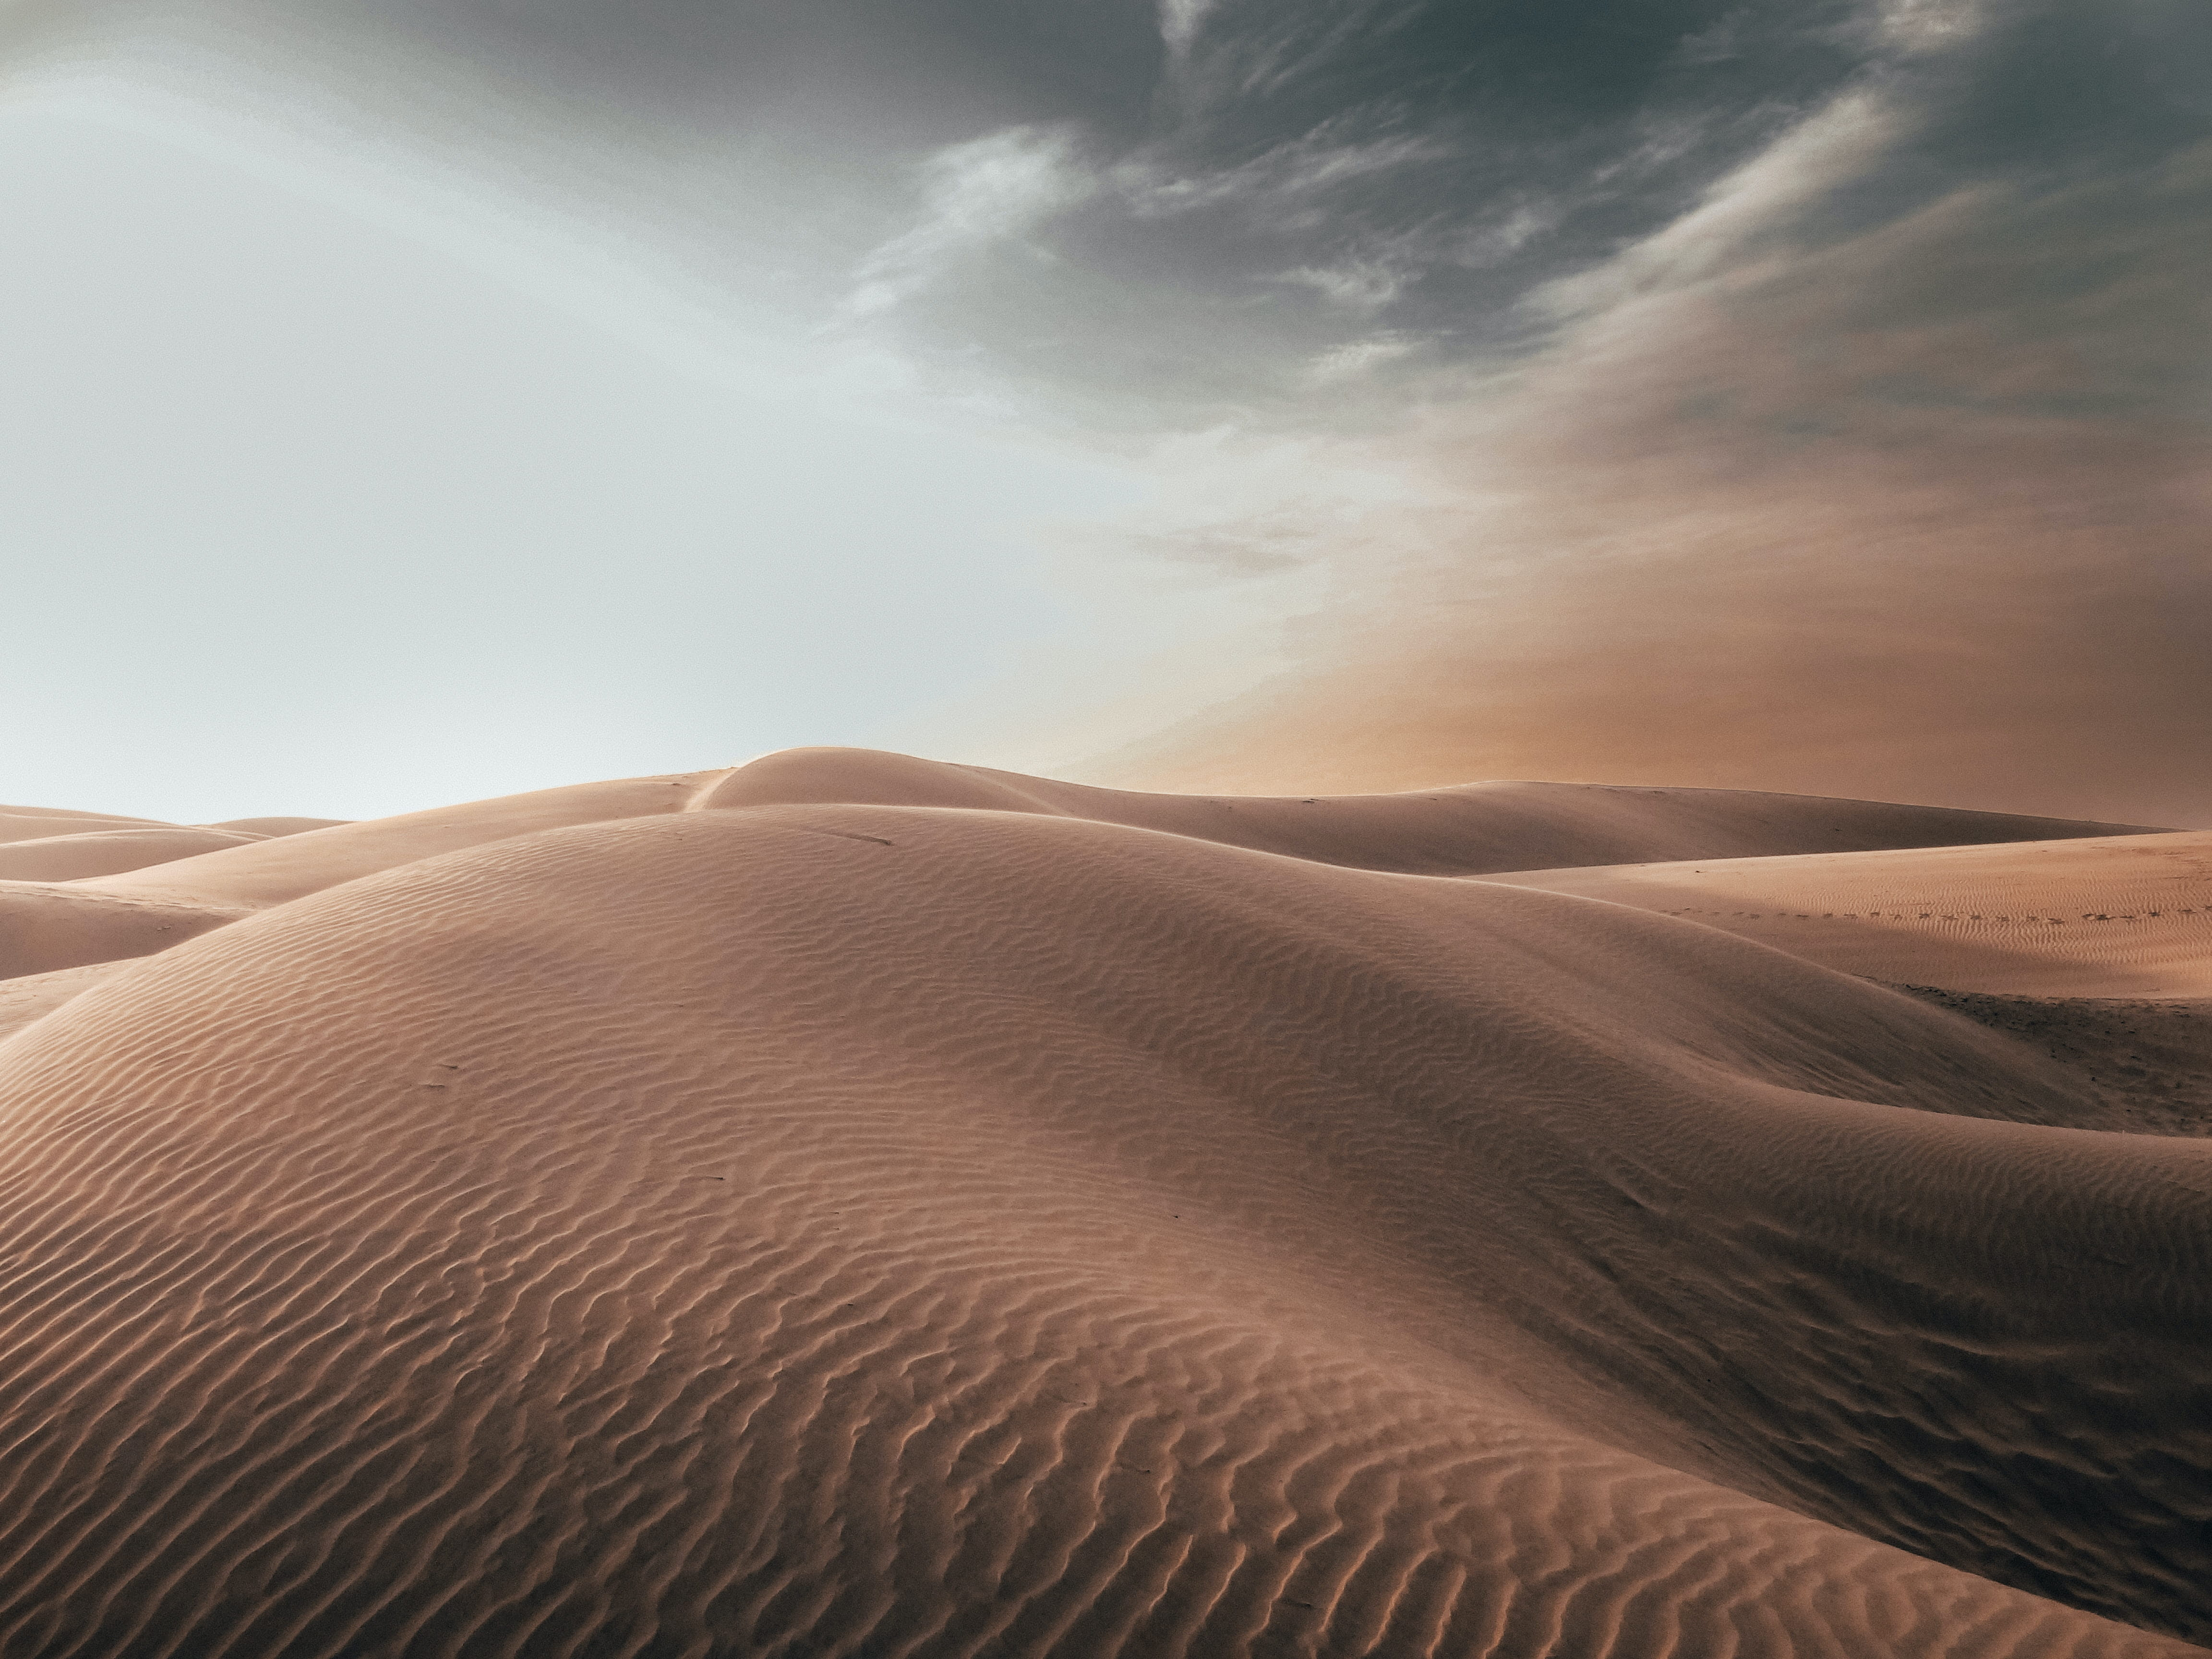
\includegraphics[width=\paperwidth]{duneslides-logo}
}
\begin{frame}[plain,noframenumbering]

	\color{c++reviewduneblue}

	\begin{flushleft}\bfseries\scshape\huge
		Richards model for simulations of water infiltration in agricultural soil using DuMu\textsuperscript{x}
	\end{flushleft}

	\

	\

	\

	\

	\

	\

	\begin{minipage}{0.47\textwidth}
		\begin{figure}[ht!]
			\centering
			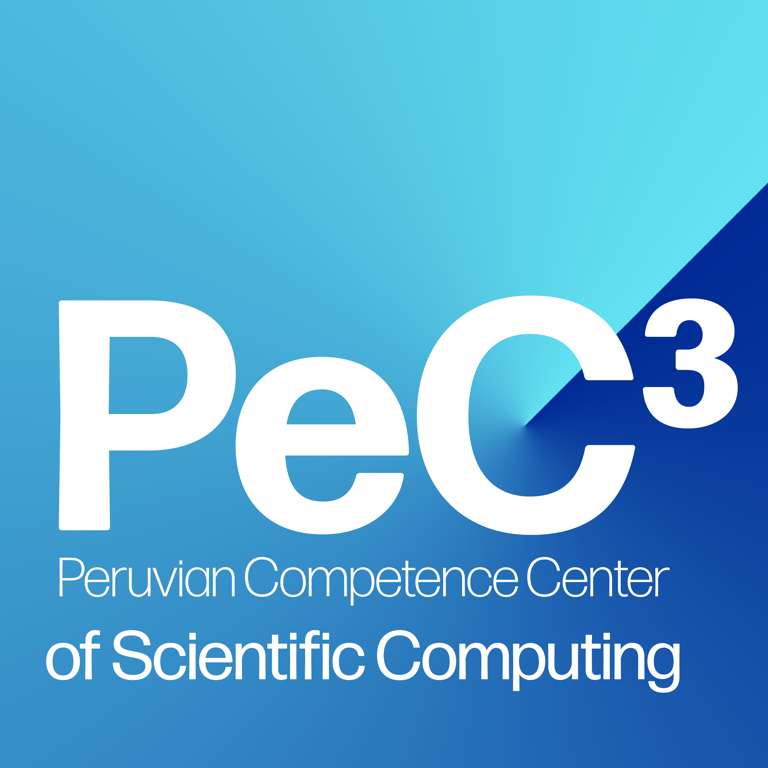
\includegraphics[height=2.5cm]{pec3}
			\caption*{
				\large
				\bfseries
				\textcolor{c++reviewduneblue}{
					Peruvian Conference on Scientific Computing
					October 4, 2022}
			}
		\end{figure}
	\end{minipage}
	\begin{minipage}{0.5\textwidth}
		\begin{flushright}
			\large
			\bfseries
			Made by\\
			John J. Leal Gomez\\
			Guillermo A. Martínez Girón\\
			Arley Martinez Jaramillo\\
			Universidad Nacional de Colombia\\
			Carlos Alonso Aznarán Laos\\
			Universidad Nacional de Ingeniería, Peru
		\end{flushright}
	\end{minipage}
	\note{
		En este webinar se presenta en dos partes, por un lado presentaremos el libro: \emph{Las matemáticas en la vida real, introducción básica al modelamiento matemático} y en segundo lugar se hará una presentación de la biblioteca modular DUNE.
	}
\end{frame}
}